\documentclass{article}
\usepackage[utf8x]{inputenc}
\usepackage{ucs}
\usepackage{amsmath} 
\usepackage{amsfonts}
\usepackage{marvosym}
\usepackage{wasysym}
\usepackage{upgreek}
\usepackage[english,russian]{babel}
\usepackage{graphicx}
\usepackage{float}
\usepackage{textcomp}
\usepackage{hyperref}
\usepackage{geometry}
  \geometry{left=2cm}
  \geometry{right=1.5cm}
  \geometry{top=1cm}
  \geometry{bottom=2cm}
\usepackage{tikz}
\usepackage{ccaption}
\usepackage{multicol}
\usepackage{hyperref}


\usepackage{listings}
%\setlength{\columnsep}{1.5cm}
%\setlength{\columnseprule}{0.2pt}

\usepackage[absolute]{textpos}



\begin{document}
\pagenumbering{gobble}
\lstset{
  language=C,                % choose the language of the code
  basicstyle=\linespread{1.1}\ttfamily,
  columns=fixed,
  fontadjust=true,
  basewidth=0.5em,
  keywordstyle=\color{blue}\bfseries,
  commentstyle=\color{gray},
  stringstyle=\ttfamily\color{orange!50!black},
  showstringspaces=false,
  numbersep=5pt,
  numberstyle=\tiny\color{black},
  numberfirstline=true,
  stepnumber=1,                   % the step between two line-numbers.        
  numbersep=10pt,                  % how far the line-numbers are from the code
  backgroundcolor=\color{white},  % choose the background color. You must add \usepackage{color}
  showstringspaces=false,         % underline spaces within strings
  captionpos=b,                   % sets the caption-position to bottom
  breaklines=true,                % sets automatic line breaking
  breakatwhitespace=true,         % sets if automatic breaks should only happen at whitespace
  xleftmargin=.2in,
  extendedchars=\true,
  keepspaces = true,
}
\lstset{literate=%
   *{0}{{{\color{red!20!violet}0}}}1
    {1}{{{\color{red!20!violet}1}}}1
    {2}{{{\color{red!20!violet}2}}}1
    {3}{{{\color{red!20!violet}3}}}1
    {4}{{{\color{red!20!violet}4}}}1
    {5}{{{\color{red!20!violet}5}}}1
    {6}{{{\color{red!20!violet}6}}}1
    {7}{{{\color{red!20!violet}7}}}1
    {8}{{{\color{red!20!violet}8}}}1
    {9}{{{\color{red!20!violet}9}}}1
}

\title{Семинар \#3: Массивы. Классные задачи.\vspace{-5ex}}\date{}\maketitle
\section*{Объявление, инициализация и присваивание:}
\begin{lstlisting}
#include <stdio.h>
int main() 
{
	// Массив из 10 чисел типа int. Без инициализации ( значения могут быть какими угодно )
	int a[10];
	// Упрощенно можно считать, что мы создали сразу 10 переменных типа int под именами
	// a[0], a[1], a[2], ... a[9]
	// Считаем числа в массив с помощью scanf
	for (int i = 0; i < 10; i++)
		scanf("%d", &a[i]);
	// Если вы знаете, что будет хранится в массиве, то можно сразу его инициализировать
	int b[10] = {6, 43, 11, 57, 91} // (оставшиеся 5 чисел будут установлены нулями)
	int c[] = {5, 4, 7}; // Размер массива будет автоматически установлен как 3
	с = {8, 7, 9};//Это ошибка! Фигурными скобачками можно пользоваться только при создании
}
\end{lstlisting}
\begin{enumerate}
\item \textbf{Инициализация:} Объявить массив под названием \texttt{numbers} с 100 элементами типа \texttt{int} и инициализировать его следующими значениями: 4, 8, 15, 16, 23, 42, все остальные элементы -- нули.
\item \textbf{Печать:} Напечатать содержимое массива numbers на экран (все 100 чисел). Числа должны быть напечатаны в одну строку через пробел.
\item \textbf{Изменить} значение 70-го элемента с нуля на 123. Проверить изменения, напечатав массив на экран.
\item \textbf{Без инициализации:} Объявите массив из 100 элементов без инициализации и напечатайте его.
\item \textbf{Нулевая инициализации:} Объявите массив из 100 элементов, проинициализировав их все нулями и напечатайте его.
\item \textbf{Присваивание:} Задать массив \texttt{numbers} квадратами номера элемента и распечатать его.
\end{enumerate}

\section*{Основные алгоритмы:}
Пример программы, которая считывает массив и печатает максимальный элемент.
\begin{lstlisting}
#include <stdio.h>
#define MAXSIZE 1000
int main() 
{
	int n;
	scanf("%d", &n);
	int array[MAXSIZE];
	for (int i = 0; i < n; i++)
		scanf("%d", &array[i]);
	int max = array[0];
	for (int i = 1; i < n; ++i)
		if (array[i] > max)
			max = array[i];
	printf("Maximum element = %d\n", max);
}
\end{lstlisting}
\begin{itemize}
\item \texttt{\#define MAXSIZE 1000} - Задаём константу-макрос MAXSIZE = 1000
\item Дальше мы считываем \texttt{n} - число элементов массива. Затем, в цикле, считываем \texttt{n} элементов.  Мы будем использовать первые \texttt{n} элементов массива. Остальные \texttt{(MAXSIZE - n)} элементы использовать не будем. Понятно, что \texttt{n} должно быть меньше либо равно \texttt{MAXSIZE}.
\item Алгоритм вычисления максимума -- проходим по массиву, храня максимальный элемент из пройденых элементов массива.
\end{itemize}

\subsection*{Задачи:}
\begin{enumerate}
\item \textbf{Сумма:} Написать программу, которая будет считывать массив и печатать сумму всех элементов.
\item \textbf{Каждый второй:} Написать программу, которая будет печатать каждый второй элемент массива.
\item \textbf{Синусы:} На вход подаётся число \texttt{n} и, затем, n углов(в радианах). Напечатать синусы этих углов. Использовать тип \texttt{float}. (Не забудьте \texttt{math.h} и опцию \texttt{-lm} для \texttt{gcc}.)
\item \textbf{Перестановка:} Напишите программу, которая будет перестанавливать 2 элемента. На вход идут количество элементов, сами элементы и 2 индекса (номера) элементов, которые нужно переставить. Например при входе:
\begin{verbatim}
4
2 4 8 16
0 2
\end{verbatim}
Должно напечатать \texttt{8 4 2 16}.
\end{enumerate}

\section*{Передача массивов в функцию}
\begin{lstlisting}
#include <stdio.h>
// Массивы в функцию всегда передаются через указатель (int arr[] и int* arr одно и то же)
void print_array(int* arr, int n) 
{
	for (int i = 0; i < n; i++)
		printf("%d ", arr[i]);
	printf("\n");
}
// Следовательно, при изменении массива в функции, он меняется и вне функции
void square_array(int arr[], int n) 
{
	for (int i = 0; i < n; i++)
		arr[i] = arr[i] * arr[i];
}
int main() 
{
	// Часто, мы не знаем размер массива заранее, поэтому берём с запасом 
	// (1000 элементов) и работаем только с n первыми элементами
	int a[1000];
	int n;
	scanf("%d", &n);
	for (int i = 0; i < n; i++)
		scanf("%d", &a[i]);
	print_array(a, n);
	square_array(a, n);
	print_array(a, n);
}
\end{lstlisting}
\begin{enumerate}
\item \textbf{Сумма массива:} Написать функцию \texttt{int sum(int* arr, int n)}, которая будет возвращать сумму массива целых чисел. Входные параметры такие же как и предыдущей задаче. Функция не должна ничего печатать и считывать. Использовать эту функцию в функции main() чтобы найти сумму чисел массива.

\item \textbf{Сумма подмассива:} Написать функцию \texttt{int sum(int* arr, int lo, int hi)}, которая будет возвращать сумму подмассива \texttt{[lo:hi]}. Функция не должна ничего печатать и считывать. Использовать эту функцию в функции main().
\begin{center}
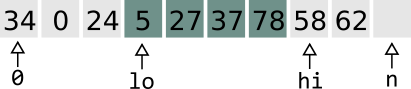
\includegraphics[scale=0.86]{../images/subarray.png}
\end{center}
\item \textbf{Умножение массива:} Написать функцию \texttt{void multiply(float* arr, int n, float k)}, которая будет умножать все элементы массива на число \texttt{k}. Протестируйте эту функцию в \texttt{main}.

\item \textbf{Индекс минимального элемента:} Написать функцию \texttt{int min\_index(int* arr, int n)}, которая будет возвращать \textit{индекс} наименьшего числа в массиве. Входные параметры такие же как и предыдущей задаче. Функция не должна ничего печатать и считывать. Если в массиве есть несколько минимальных элементов, то функция должна вернуть индекс первого из них.
\end{enumerate}

\section*{Сортировка выбором}
\begin{enumerate}
\item \textbf{Сортировка выбором:} Написать функцию \texttt{void selection\_sort(int* arr, int n)}, которая будет сортировать массив методом выбора. \\
Алгоритм сортировки методом выбора:
\begin{itemize}
\item Идём циклом с индексом \texttt{i} от \texttt{0} \texttt{до} \texttt{n}.\\
\begin{itemize}
\item Находим индекс минимального элемента от \texttt{i} до \texttt{n}.\\
\item Переставляем местами элемент с индексом \texttt{i} и этот минимальный элемент\\
\end{itemize}
\end{itemize}
Протестируйте работу функции на массиве из хотя бы 15-ти элементов.
\begin{lstlisting}
#include <stdio.h>
#define MAXSIZE 100
// Тут Вам нужно написать функции print_array и selection_sort:
...
int main() 
{
	int a[MAXSIZE] = {86, 12, 44, -36, -32, 2, -10, -3, 39, 60, 79, 97, -17, -29, 93};
	print_array(a, 0, 15);
	selection_sort(a, 15);
	print_array(a, 0, 15);
}
\end{lstlisting}



\item \textbf{Сортировка выбором по убыванию:} Написать функцию \texttt{void selection\_sort\_descend(int* arr, int n)}, которая будет сортировать массив методом выбора по убыванию.

\item \textbf{Рекурсивная сортировка выбором:} Написать функцию \texttt{void selection\_sort\_rec(int* arr, int lo, int hi)}, которая будет сортировать часть массива от индекса \texttt{lo} до \texttt{hi} (не включая \texttt{hi}) методом выбора. Используйте рекурсию.
Алгоритм сортировки методом выбора для сортировки подмассива \texttt{[lo:hi]}:
\begin{itemize}
\item Если \texttt{hi - lo <= 1} (один элемент), то завершаем функцию (просто \texttt{return}).
\item Находим индекс минимального элемента в подмассиве \texttt{[lo:hi]} 
\item Переставляем местами элемент с индексом \texttt{lo} и минимальный элемент
\item Повторяем то же самое для подмассива \texttt{[lo+1:hi]} 
\end{itemize}
\end{enumerate}
\newpage


\section*{Двумерные массивы}
\begin{lstlisting}
#include <stdio.h>
#define MAX 100
void print_array(int arr[MAX][MAX], int n, int m) 
{
	for (int i = 0; i < n; i++) {
		for (int j = 0; j < m; j++)
			printf("%d ", arr[i][j]);
		printf("\n");
	}
}
int main() 
{
	// Создаём массивы с запасом
	int a[MAX][MAX] = {{7, 7, 2}, {1, 8, 3}, {2, 1, 6}};
	int b[MAX][MAX] = {{5, 2, 9}, {-4, 2, 11}, {7, 1, -5}};
	// Печатаем только 9 элементов
	print_array(a, 3, 3);
}
\end{lstlisting}
\begin{enumerate}
\item \textbf{Умножение на число:} Написать
\texttt{void multiply\_num(int arr[MAX][MAX], int n, int m, int x)}\\
которая будет умножать двумерный массив на число.
\item \textbf{Сложение:} Написать
\texttt{void sum(int A[MAX][MAX], int B[MAX][MAX], int C[MAX][MAX], int n, int m)}\\
которая будет складывать матрицы и записывать их в \texttt{C}.
\item \textbf{Умножение:} Написать
\texttt{void mult(int A[MAX][MAX], int B[MAX][MAX], int C[MAX][MAX],int n, int m)}\\
которая будет перемножать матрицы \texttt{A} и \texttt{B} (строка на столбец) и записывать их в массив \texttt{C}.

\iffalse
\item \textbf{N-я степень:} Написать
\texttt{void power(int A[MAX][MAX], int B[MAX][MAX], int n, int m, int N)}\\
которая будет возводить матрицу \texttt{A} в степень \texttt{N} и записывать результат в массив \texttt{B}.
\fi
\end{enumerate}

\section*{Считывание из файла}
Пример программы, которая считывает массив из файла и печатает его содержимое на экран (нужно создать файл \texttt{input.txt} с входными данными в вашей рабочей папке):
\begin{lstlisting}
#include <stdio.h>
#define MAX 100
int main() 
{
    FILE* file = fopen("input.txt", "r");  // "r" -- read   "w" -- write
    int n;
    fscanf(file, "%d", &n); // fscanf(file, < то же самое, что и в scanf >
    int array[MAX];
    for (int i = 0; i < n; i++)
        fscanf(file, "%d", &array[i]);
    
    for (int i = 0; i < n; i++)
        printf("%d ", array[i]);
    fclose(file);
}
\end{lstlisting}
\begin{enumerate}
\item \textbf{Сортировка из файла:} Написать программу, которая будет считывать массив чисел из файла \texttt{numbers.txt} и записывать в файл \texttt{sorted.txt} отсортированные числа.
\item \textbf{Умножение матриц из файла:} Написать программу, которая будет считывать матрицы из файлов \texttt{mat1.txt} и \texttt{mat2.txt}, перемножать их и записывать в файл \texttt{mult.txt}.
\end{enumerate}
\end{document}